\documentclass[12pt]{article}
\usepackage{amsmath}
\usepackage{amssymb}
\usepackage{bm}
\usepackage{graphicx}
\usepackage{epstopdf}
\usepackage{xcolor}
\usepackage{hyperref}
\DeclareGraphicsRule{.tif}{png}{.png}{`convert #1 `basename #1 .tif`.png}
\usepackage{color}
\pagestyle{plain}
\usepackage{longtable}
\usepackage{textcomp}
\graphicspath{{../../../etc/plots/climate_et/test_plots/}}

\RequirePackage{natbib}
\bibliographystyle{agufull08}

% Bib aliases
\makeatletter
\def\@citex[#1]#2{\leavevmode
  \let\@citea\@empty
  \@cite{\@for\@citeb:=#2\do
    {\@citea\def\@citea{,\penalty\@m\ }%
\edef\magic##1{\let##1\expandafter\noexpand\csname bibalias@\@citeb\endcsname}%
\magic\tmp \ifx\tmp\relax\else \let\@citeb\tmp\fi
     \edef\@citeb{\expandafter\@firstofone\@citeb\@empty}%
     \if@filesw\immediate\write\@auxout{\string\citation{\@citeb}}\fi
     \@ifundefined{b@\@citeb}{\hbox{\reset@font\bfseries ?}%
       \G@refundefinedtrue
       \@latex@warning
         {Citation `\@citeb' on page \thepage \space undefined}}%
       {\@cite@ofmt{\csname b@\@citeb\endcsname}}}}{#1}}
\def\bibalias#1#2{\expandafter\def\csname bibalias@#1\endcsname{#2}}
\makeatother

\title{Supplementary material: When does vapor pressure deficit drive or
  reduce evapotranspiration?}

\author{Adam Massmann, Pierre Gentine, and Changjie Lin}

\date{\today}

\begin{document}

\maketitle

The manuscript analyzes the partial derivative of ET with respect to
VPD. This assumes that all other quantities remain fixed, including the
plant parameters g$_1$ and uWUE (and by extension, $\lambda$). In
reality, these parameters may vary with environmental conditions, and
specifically soil moisture. However because soil moisture
\textit{only} enters the partial derivative directly through these
plant terms, if the plant parameters are weak functions of soil
moisture then the theory can be directly applied to a broader range of
conceptual VPD scenarios, including observed compound events between
high VPD and low soil moisture \citep{Zhou_2019}. To help the reader
assess the soil moisture dependence of uWUE (and partially by
extension $\lambda$ and g$_1$), we provide here figures showing the
distribution of uWUE with SWC for each of 66 FLUXNET sites from the
FLUXNET-2015 database. The functional relationship between uWUE and
SWC varies, with a mix of sites showing strong and weak
SWC-dependence. For all sites the ratio of signal to noise is very
low, an unfortunate consequence of taking a ratio of two highly
uncertain eddy-covariance derived fluxes. In general we find this
analysis inconclusive.

The paper does not rely on assumptions about uWUE's functional
relationship with soil moisture so we do not include the figures in
the body of the manuscript. But given that constant uWUE and g$_1$
assumptions can make our theory more useful to the reader we provide
the figures for their interpretation, and motivation for future
research.

Additionally, we include a figure showing the joint distribution
between saturation vapor pressure and relative humidity calculated
from the FLUXNET-2015 data. Relative humidity and saturation vapor
pressure are much more independent than saturation vapor pressure and
VPD, and we use an assumption that relative humidity and saturation
vapor pressure can be approximated as independent in order to evaluate
$\frac{\partial ET}{\partial VPD}$. Please note that at a given site,
the relationship may be more or less independent depending on the
hydroclimate.

\section{Description of data}
\subsection{Data}
\label{data}
We use both meteorological and eddy-covariance data from the
FLUXNET2015 database (data available at \sloppy
\url{https://fluxnet.fluxdata.org/data/fluxnet2015-dataset/} \sloppy),
including all Tier 1 sites with at least four years of data. Sixty-six
sites met these requirements, and were grouped into nine plant
functional types (PFT) according to the International
Geosphere-Biosphere Programme vegetation classification scheme
\citep{Loveland_1999}: cropland (CRO), grass (GRA), deciduous
broadleaf forest (DBF), evergreen broadleaf forest (EBF), evergreen
needleleaf forest (ENF), mixed forest (MF), closed shrub (CSH),
savannah (SAV), and woody savannah (WSA).

\begin{figure}[h]
  \centering 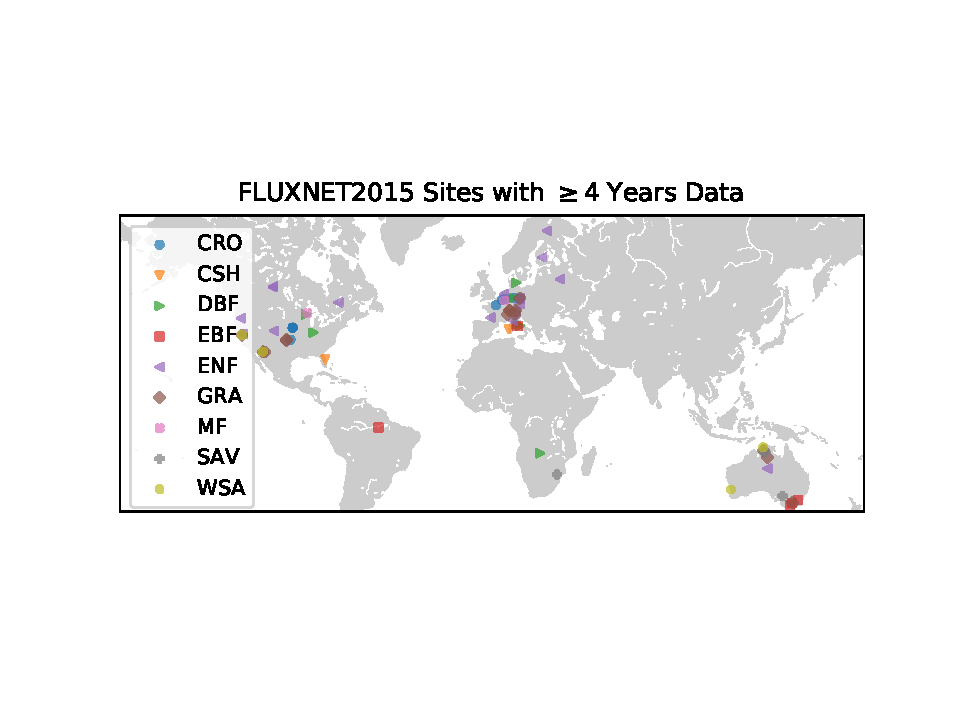
\includegraphics[trim={0 3cm 0 3cm}, clip]{./map.pdf}
  \caption{Plant functional type and location of FLUXNET2015 sites
    used in this analysis.}
  \label{map_fig}
\end{figure}
We filter and quality control the FLUXNET-2015 data using a similar
procedure as \cite{Zhou_2015}:

\begin{itemize}
\item Only measured or highest (``good'') quality gapfilled data,
  according to quality control flags, are used.
\item To isolate the growing season, we only use days in which the
  average Gross Primary Productivity (GPP) exceeds 10\% of the
  observed 95th percentile of GPP for a given site. GPP is calculated
  using the nighttime respiration partitioning method.
\item We remove days with rain and the day following to avoid issues
  with rain interception and sensor saturation at high relative
  humidity (\cite{Medlyn_2017}).
\item For SWC measurements, we use the shallowest observed layer
  available at each site.
\end{itemize}

Additionally, as in \citet{Lin_2018}, we restrict data to the daytime,
which is identified when downwelling shortwave radiation is greater
than 50 W m$^{-2}$ and sensible heat flux is greater than 5 W
m$^{-2}$. To reduce the chance of sensor saturation at high relative
humidity, we remove all time steps for which VPD is less than .01 kPa,
and to reduce errors at low windspeeds we remove all periods with wind
magnitudes less than 0.5 m s$^{-1}$. Timesteps with negative observed
GPP or ET are also removed, and we aggregate half hourly data to
hourly averages to reduce noise \citep{Lin_2018}.  After these quality
control procedures, 400,983 upscaled hourly observations remain.


\begin{figure}
  \centering \includegraphics{./supp-figs/0joint_rh_es.pdf}
  \caption{The joint distribution of relative humidity and saturation
    vapor pressure for the FLUXNET2015 dataset.}
  \end{figure}

\input{supp-figs.tex}


\section{FLUXNET2015 sites}
  % below taken adapted from Trevor Keenan's FLUXNET citations
  % at github.com/trevorkeenan/FLUXNET_citations
  Table A1: Metadata and citations for flux sites used in this analysis. All data are gathered from \url{www.fluxdata.org}, and citations are aggregated using tools available at \url{https://github.com/trevorkeenan/FLUXNET_citations}.
  \begin{longtable}{l l l l l l l}
    \hline
    \textbf{Site} &
    \textbf{PFT} &
    \textbf{Lat} &
    \textbf{Lon} &
    \textbf{Clim\textsuperscript{1}} &
    \textbf{Period} &
    \textbf{References} \\
    [0.5ex]
    \hline
    AT-Neu & GRA & 47.1167 & 11.3175 & Unk & 2002-2012 & \cite{AT-Neu} \\
AU-ASM & ENF & -22.2830 & 133.2490 & Unk & 2010-2013 & \cite{AU-ASM} \\
AU-Cpr & SAV & -34.0021 & 140.5891 & Unk & 2010-2014 & \cite{AU-Cpr} \\
AU-DaP & GRA & -14.0633 & 131.3181 & Aw  & 2007-2013 & \cite{AU-DaP} \\
AU-DaS & SAV & -14.1593 & 131.3881 & Aw  & 2008-2014 & \cite{AU-DaS} \\
AU-Dry & SAV & -15.2588 & 132.3706 & Unk & 2008-2014 & \cite{AU-Dry} \\
AU-Gin & WSA & -31.3764 & 115.7138 & Unk & 2011-2014 & \cite{AU-Gin} \\
AU-How & WSA & -12.4943 & 131.1523 & Aw  & 2001-2014 & \cite{AU-How} \\
AU-Rig & GRA & -36.6499 & 145.5759 & Unk & 2011-2014 & \cite{AU-Gin} \\
AU-Stp & GRA & -17.1507 & 133.3502 & Unk & 2008-2014 & \cite{AU-DaP} \\
AU-Tum & EBF & -35.6566 & 148.1517 & Cfb & 2001-2014 & \cite{AU-Tum} \\
AU-Whr & EBF & -36.6732 & 145.0294 & Unk & 2011-2014 & \cite{AU-Whr} \\
AU-Wom & EBF & -37.4222 & 144.0944 & Unk & 2010-2012 & \cite{AU-Wom} \\
BE-Lon & CRO & 50.5516 & 4.7461 & Cfb & 2004-2014 & \cite{BE-Lon} \\
BE-Vie & MF & 50.3051 & 5.9981 & Cfb & 1996-2014 & \cite{BE-Vie} \\
BR-Sa3 & EBF & -3.0180 & -54.9714 & Am & 2000-2004 & \cite{BR-Sa3} \\
CA-Qfo & ENF & 49.6925 & -74.3421 & Dfc & 2003-2010 & \cite{CA-Qfo} \\
CA-SF1 & ENF & 54.4850 & -105.8176 & Dfc & 2003-2006 & \cite{CA-SF1} \\
CA-SF2 & ENF & 54.2539 & -105.8775 & Dfc & 2001-2005 & \cite{CA-SF1} \\
CH-Cha & GRA & 47.2102 & 8.4104 & Unk & 2005-2014 & \cite{CH-Cha} \\
CH-Dav & ENF & 46.8153 & 9.8559 & Unk & 1997-2014 & \cite{CH-Dav} \\
CH-Fru & GRA & 47.1158 & 8.5378 & Unk & 2005-2014 & \cite{CH-Fru} \\
DE-Geb & CRO & 51.1001 & 10.9143 & Unk & 2001-2014 & \cite{DE-Geb} \\
DE-Gri & GRA & 50.9500 & 13.5126 & Cfb & 2004-2014 & \cite{DE-Gri} \\
DE-Hai & DBF & 51.0792 & 10.4530 & Unk & 2000-2012 & \cite{DE-Hai} \\
DE-Kli & CRO & 50.8931 & 13.5224 & Cfb & 2004-2014 & \cite{DE-Gri} \\
DE-Lkb & ENF & 49.0996 & 13.3047 & Unk & 2009-2013 & \cite{DE-Lkb} \\
DE-Obe & ENF & 50.7867 & 13.7213 & Cfb & 2008-2014 & {\textendash} \\
DE-Seh & CRO & 50.8706 & 6.4497 & Unk & 2007-2010 & \cite{DE-Seh} \\
DE-Tha & ENF & 50.9624 & 13.5652 & Cfb & 1996-2014 & \cite{DE-Tha} \\
DK-Sor & DBF & 55.4859 & 11.6446 & Unk & 1996-2014 & \cite{DK-Sor} \\
FI-Hyy & ENF & 61.8474 & 24.2948 & Unk & 1996-2014 & \cite{FI-Hyy} \\
FI-Sod & ENF & 67.3619 & 26.6378 & Unk & 2001-2014 & \cite{FI-Sod} \\
FR-Gri & CRO & 48.8442 & 1.9519 & Cfb & 2004-2013 & \cite{FR-Gri} \\
FR-LBr & ENF & 44.7171 & -0.7693 & Unk & 1996-2008 & \cite{FR-LBr} \\
IT-Col & DBF & 41.8494 & 13.5881 & Unk & 1996-2014 & \cite{IT-Col} \\
IT-Cpz & EBF & 41.7052 & 12.3761 & Unk & 1997-2009 & \cite{IT-Cpz} \\
IT-Lav & ENF & 45.9562 & 11.2813 & Unk & 2003-2014 & \cite{IT-Lav} \\
IT-MBo & GRA & 46.0147 & 11.0458 & Unk & 2003-2013 & \cite{IT-MBo} \\
IT-Noe & CSH & 40.6061 & 8.1515 & Unk & 2004-2014 & \cite{IT-Noe} \\
IT-Ren & ENF & 46.5869 & 11.4337 & Unk & 1998-2013 & \cite{IT-Ren} \\
IT-Ro2 & DBF & 42.3903 & 11.9209 & Unk & 2002-2012 & \cite{IT-Ro2} \\
IT-SRo & ENF & 43.7279 & 10.2844 & Unk & 1999-2012 & \cite{IT-SRo} \\
IT-Tor & GRA & 45.8444 & 7.5781 & Unk & 2008-2014 & \cite{IT-Tor} \\
NL-Loo & ENF & 52.1666 & 5.7436 & Unk & 1996-2013 & \cite{NL-Loo} \\
RU-Fyo & ENF & 56.4615 & 32.9221 & Unk & 1998-2014 & \cite{RU-Fyo} \\
US-AR1 & GRA & 36.4267 & -99.4200 & Dsa & 2009-2012 & \cite{US-AR1} \\
US-AR2 & GRA & 36.6358 & -99.5975 & Dsa & 2009-2012 & \cite{US-AR1} \\
US-ARM & CRO & 36.6058 & -97.4888 & Cfa & 2003-2012 & \cite{US-ARM} \\
US-Blo & ENF & 38.8953 & -120.6328 & Csa & 1997-2007 & \cite{US-Blo} \\
US-KS2 & CSH & 28.6086 & -80.6715 & Cwa & 2003-2006 & \cite{US-KS2} \\
US-MMS & DBF & 39.3232 & -86.4131 & Cfa & 1999-2014 & \cite{US-MMS} \\
US-Me2 & ENF & 44.4523 & -121.5574 & Csb & 2002-2014 & \cite{US-Me2} \\
US-NR1 & ENF & 40.0329 & -105.5464 & Dfc & 1998-2014 & \cite{US-NR1} \\
US-Ne1 & CRO & 41.1651 & -96.4766 & Dfa & 2001-2013 & \cite{US-Ne1} \\
US-Ne2 & CRO & 41.1649 & -96.4701 & Dfa & 2001-2013 & \cite{US-Ne1} \\
US-Ne3 & CRO & 41.1797 & -96.4397 & Dfa & 2001-2013 & \cite{US-Ne1} \\
US-SRG & GRA & 31.7894 & -110.8277 & Bsk & 2008-2014 & \cite{US-SRG} \\
US-SRM & WSA & 31.8214 & -110.8661 & Bsk & 2004-2014 & \cite{US-SRM} \\
US-Syv & MF & 46.2420 & -89.3477 & Dfb & 2001-2014 & \cite{US-Syv} \\
US-Ton & WSA & 38.4316 & -120.9660 & Csa & 2001-2014 & \cite{US-Ton} \\
US-Var & GRA & 38.4133 & -120.9507 & Csa & 2000-2014 & \cite{US-Var} \\
US-WCr & DBF & 45.8059 & -90.0799 & Dfb & 1999-2014 & \cite{US-WCr} \\
US-Wkg & GRA & 31.7365 & -109.9419 & Bsk & 2004-2014 & \cite{US-Wkg} \\
ZA-Kru & SAV & -25.0197 & 31.4969 & Unk & 2000-2010 & \cite{ZA-Kru} \\
ZM-Mon & DBF & -15.4378 & 23.2528 & Unk & 2000-2009 & \cite{ZM-Mon} \\

    [1ex]
    \hline
  \end{longtable}
\textsuperscript{1} K{\"o}ppen Climate classification.

\bibliography{references}

\end{document}
